\subsection{Algoritmi di Attraversamento}
\begin{figure}[h!]
    \centering
    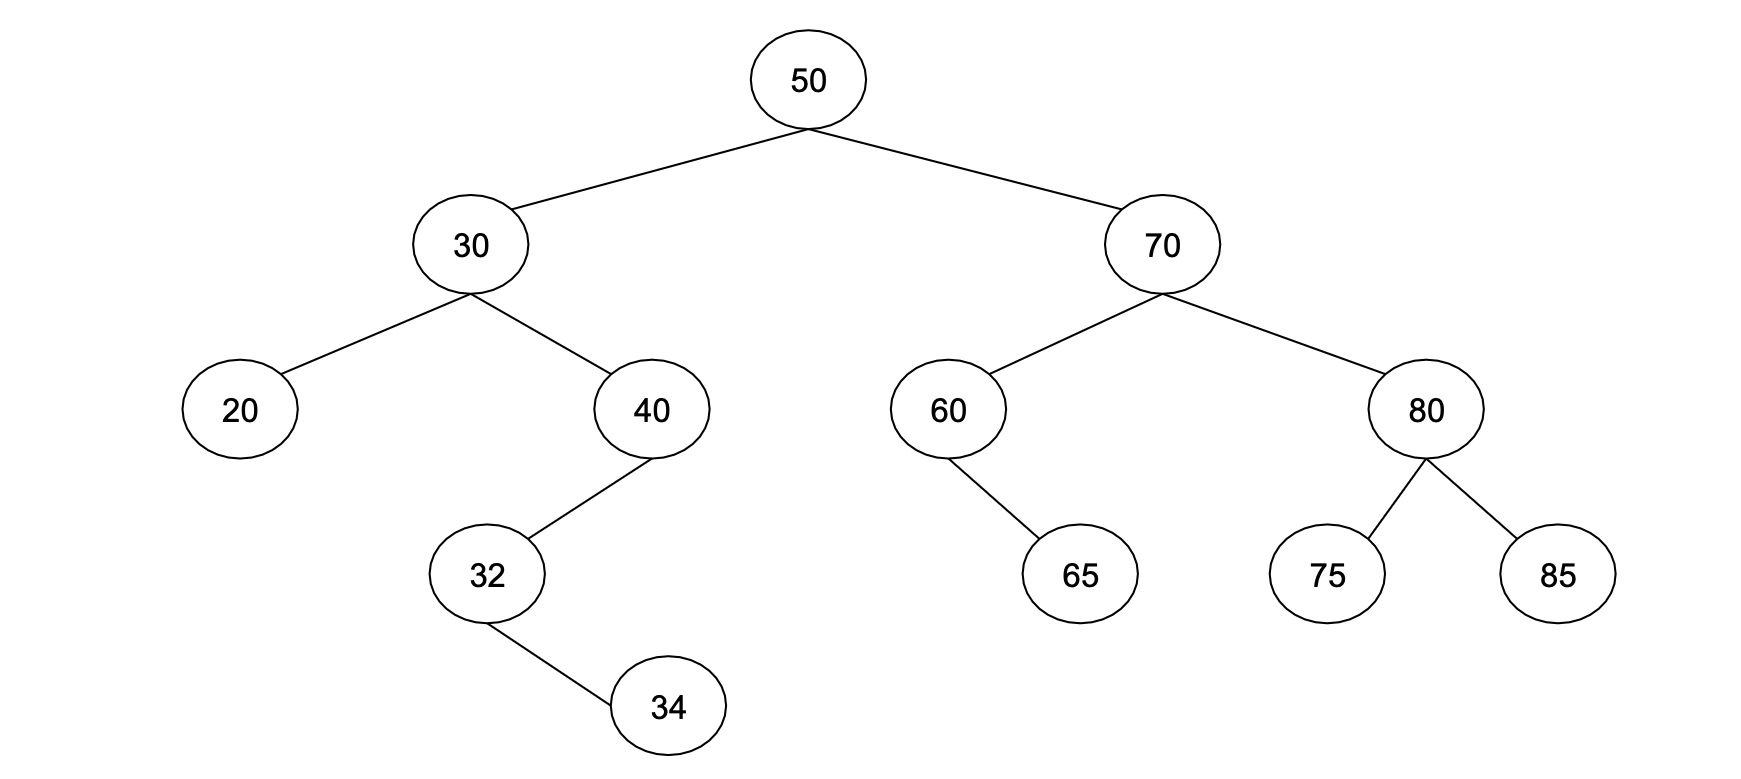
\includegraphics[width=1\textwidth]{images/bst.png}
    \caption{BST di esempio utilizzato per le operazioni.}
    \label{fig:bst_example}
\end{figure}

\begin{itemize}
    \item \textbf{Attraversamento In-Ordine (In-order Traversal)}, complessità: $\Theta(n)$
    \begin{itemize}
        \item \textbf{Descrizione:} Questo algoritmo visita un albero binario di ricerca (BST) processando prima il sottoalbero sinistro, poi la radice e infine il sottoalbero destro. Il risultato è la stampa delle chiavi dei nodi in ordine non decrescente.
        \item \textbf{Esempio:} Dato l'albero in Figura \ref{fig:bst_example}, la sequenza di output è:
        \begin{verbatim}
20, 30, 32, 34, 40, 50, 60, 65, 70, 75, 80, 85
        \end{verbatim}
    \end{itemize}

    \item \textbf{Attraversamento Pre-Ordine (Pre-order Traversal)}, complessità: $\Theta(n)$
    \begin{itemize}
        \item \textbf{Descrizione:} L'attraversamento anticipato (o pre-ordine) visita prima la radice, poi ricorsivamente il sottoalbero sinistro e infine ricorsivamente il sottoalbero destro.
        \item \textbf{Esempio:} Utilizzando lo stesso albero, l'output è:
        \begin{verbatim}
50, 30, 20, 40, 32, 34, 70, 60, 65, 80, 75, 85
        \end{verbatim}
    \end{itemize}

    \item \textbf{Attraversamento Post-Ordine (Post-order Traversal)}, complessità: $\Theta(n)$
    \begin{itemize}
        \item \textbf{Descrizione:} L'attraversamento posticipato (o post-ordine) visita ricorsivamente prima il sottoalbero sinistro, poi il sottoalbero destro e infine la radice.
        \item \textbf{Esempio:} Per lo stesso albero, la sequenza di output generata è:
        \begin{verbatim}
20, 34, 32, 40, 30, 65, 60, 75, 85, 80, 70, 50
        \end{verbatim}
    \end{itemize}

    \item \textbf{Attraversamento per Livelli (Level-order Traversal)}, complessità: $\Theta(n)$
    \begin{itemize}
        \item \textbf{Descrizione:} Questo algoritmo visita i nodi dell'albero livello per livello, da sinistra a destra, partendo dalla radice. Si avvale di una coda: la radice viene inserita in coda, e poi, in un ciclo, il nodo in testa viene rimosso, la sua chiave stampata e i suoi figli (se esistenti) vengono aggiunti alla coda.
        \item \textbf{Esempio:} Per l'albero di riferimento, l'output è: 50, 30, 70, 20, 40, 60, 80, 32, 65, 75, 85, 34.
    \end{itemize}
\end{itemize}

\subsection{Operazioni su Insiemi Dinamici (Dynamic Set Operations)}
Le operazioni su insiemi dinamici per un BST hanno una complessità temporale proporzionale all'altezza dell'albero, $h$.

\begin{itemize}
    \item \textbf{Ricerca (Search)}, complessità: $\Theta(h)$
    \begin{itemize}
        \item \textbf{Descrizione:} L'algoritmo `BST-SEARCH(T, k)` cerca un nodo con chiave `k`. Partendo dalla radice, confronta `k` con la chiave del nodo corrente. Se `k` è minore, prosegue nel sottoalbero sinistro; se è maggiore, prosegue in quello destro, fino a trovare il nodo o un puntatore `NIL`.
        \item \textbf{Esempio:} La ricerca di 65 (`BST-SEARCH(T, 65)`) esamina la sequenza di nodi: 50, 70, 60, e infine 65.
    \end{itemize}

    \item \textbf{Minimo e Massimo (Minimum \& Maximum)}, complessità: $\Theta(h)$
    \begin{itemize}
        \item \textbf{Descrizione:} `BST-MINIMUM` trova il nodo con la chiave più piccola seguendo ricorsivamente i puntatori al figlio sinistro fino a che non si trova un puntatore `NIL`. Analogamente, `BST-MAXIMUM` segue i puntatori al figlio destro per trovare la chiave massima.
        \item \textbf{Esempio:} `BST-MINIMUM(T)` restituisce il nodo con chiave 20, mentre `BST-MAXIMUM(T)` restituisce il nodo con chiave 85.
    \end{itemize}
    
    \item \textbf{Successore (Successor)}, complessità: $\Theta(h)$
    \begin{itemize}
        \item \textbf{Descrizione:} `BST-SUCCESSOR(x)` trova il nodo con la chiave più piccola che sia maggiore della chiave del nodo `x`. Se il nodo `x` ha un sottoalbero destro, il successore è il minimo di tale sottoalbero. Altrimenti, è il più basso antenato di `x` di cui `x` è discendente nel sottoalbero sinistro.
        \item \textbf{Esempio:} Il successore del nodo con chiave 40 è il nodo con chiave 50.
    \end{itemize}

    \item \textbf{Inserimento (Insert)}, complessità: $\Theta(h)$
    \begin{itemize}
        \item \textbf{Descrizione:} `BST-INSERT(T, z)` inserisce un nuovo nodo `z` mantenendo la proprietà del BST. L'algoritmo cerca la posizione corretta come in `BST-SEARCH` e, una volta trovato un puntatore `NIL`, inserisce `z` come nuova foglia in quella posizione.
        \item \textbf{Esempio:} Per inserire un nodo con chiave 31, l'algoritmo lo posiziona come figlio sinistro del nodo con chiave 32.
    \end{itemize}

    \item \textbf{Cancellazione (Delete)}, complessità: $\Theta(h)$
    \begin{itemize}
        \item \textbf{Descrizione:} `BST-DELETE(T, z)` rimuove il nodo `z`. L'operazione considera tre casi: se `z` è una foglia, viene rimosso; se ha un solo figlio, viene sostituito da esso; se ha due figli, la sua chiave viene sostituita da quella del suo successore, e il nodo successore viene rimosso (quest'ultimo ricade in uno dei primi due casi).
        \item \textbf{Esempio:} Per cancellare il nodo con chiave 70 (che ha due figli), la sua chiave viene sostituita da quella del suo successore (75). Il nodo originale contenente 75 viene poi rimosso dalla sua posizione.
    \end{itemize}
\end{itemize}